\documentclass[aps,prl,twocolumn,epsf,epsfig,amsmath]{revtex4}

\usepackage{latexsym}
\usepackage{hyperref}
\usepackage{times}
\usepackage{graphicx}
\usepackage{amsmath}
\usepackage{multirow} 
\usepackage{amsthm}
\usepackage{dcolumn}% Align table columns on decimal point
\usepackage{bm}% bold math
\usepackage{ textcomp }
\usepackage{color}
\usepackage{amssymb}
\usepackage{xcolor}
\usepackage{easyReview}
\usepackage{mathdots}
\usepackage{float}
\usepackage{lineno}
\usepackage{todonotes}
\usepackage{array}

%\usepackage{xcolor,colortbl}
\setlength{\marginparwidth}{2cm}
\newcommand{\beq}{\begin{eqnarray}}
\newcommand{\eeq}{\end{eqnarray}}
\newcommand{\Ag}{{\AA \; }} 
\newcommand{\llv}{\lVert}
\newcommand{\rrv}{\rVert}
%\renewcommand{\llll}{\langle \langle}
\newcommand{\rrr}{\rangle \rangle}
\newcommand{\disp}[1]{Eq. (\ref{#1})}
\newcommand{\dispop}[1]{ {\bf (\ref{#1})}}
\newcommand{\refdisp}[1]{Ref. [\onlinecite{#1}]}
\newcommand{\figdisp}[1]{Fig. \ref{#1}}
\newcommand{\U}{{\cal U}}
\newcommand{\bb}[1]{{{\mathbf #1}}}
\newcommand{\bg}{\mathbf{g}}
\newcommand{\pmai}[1]{\textcolor{blue}{#1}}
\begin{document}
\title{Capturing 98\% of Hubbard Mottness with a Momentum-Mixing Hatsugai–Kohmoto Model}

\author{Peizhi Mai$^{1}$}
\email{peizhimai@gmail.com}
\author{Philip W. Phillips$^{2}$}
\email{dimer@illinois.edu}


\affiliation{$^2$Department of Physics and Institute of Condensed Matter Theory, University of Illinois at Urbana-Champaign, Urbana, IL 61801, USA}



\begin{abstract}


\end{abstract}
\date{August 2025}

% Users of the {thebibliography} environment or BibTeX should use the
% scicite.sty package, downloadable from *Science* at
% www.sciencemag.org/about/authors/prep/TeX_help/ .
% This package should properly format in-text
% reference calls and reference-list numbers.



\maketitle
\section{Introduction}

 \begin{figure*}[t]
    \centering
    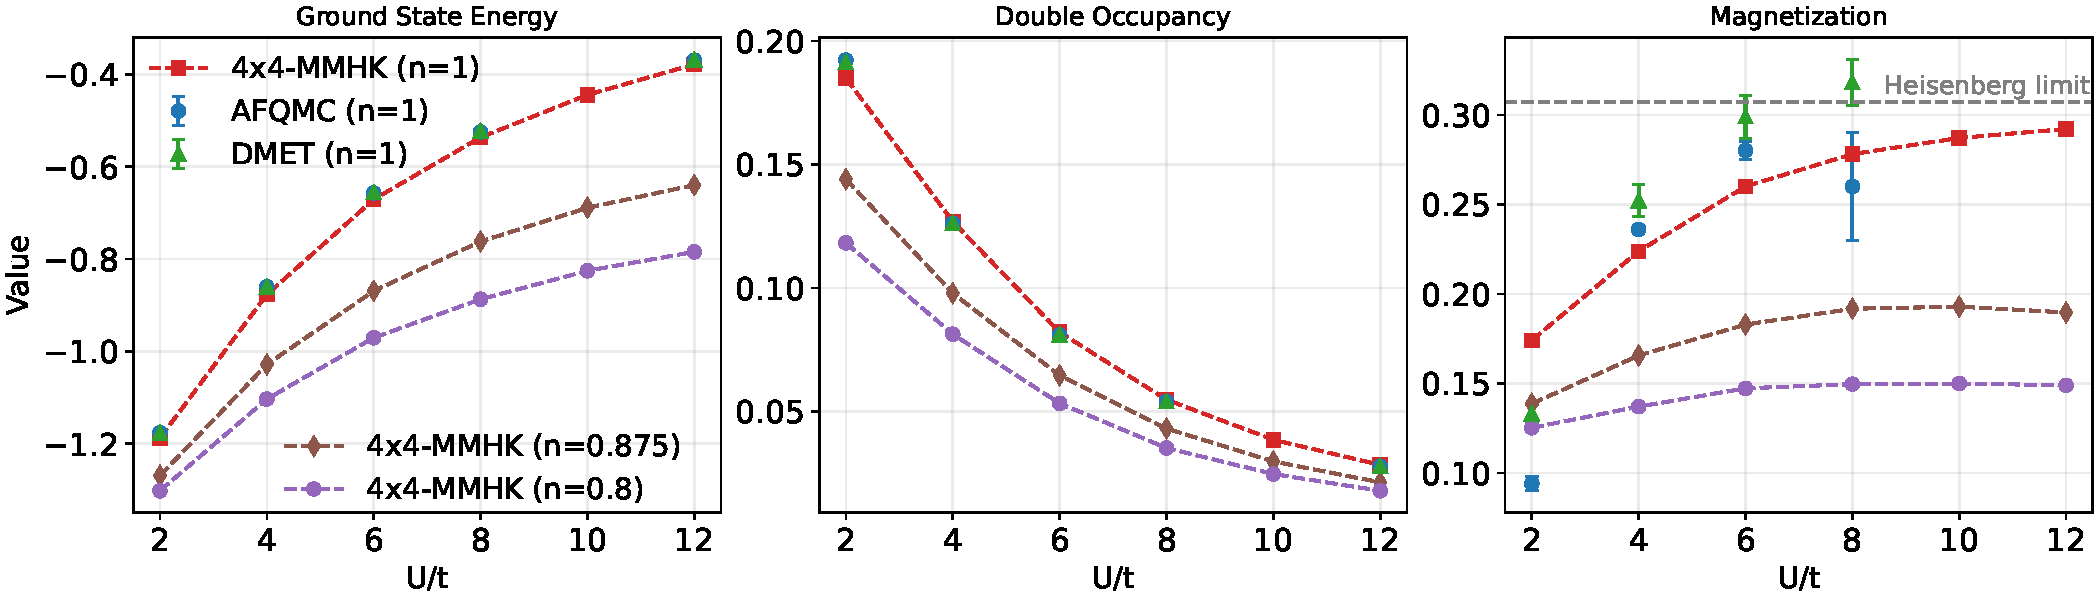
\includegraphics[width=\linewidth]{./figures/comparison.pdf}
    \caption{XXX}
    \label{fig:hfbm}
\end{figure*}


 \begin{figure}[t]
    \centering
    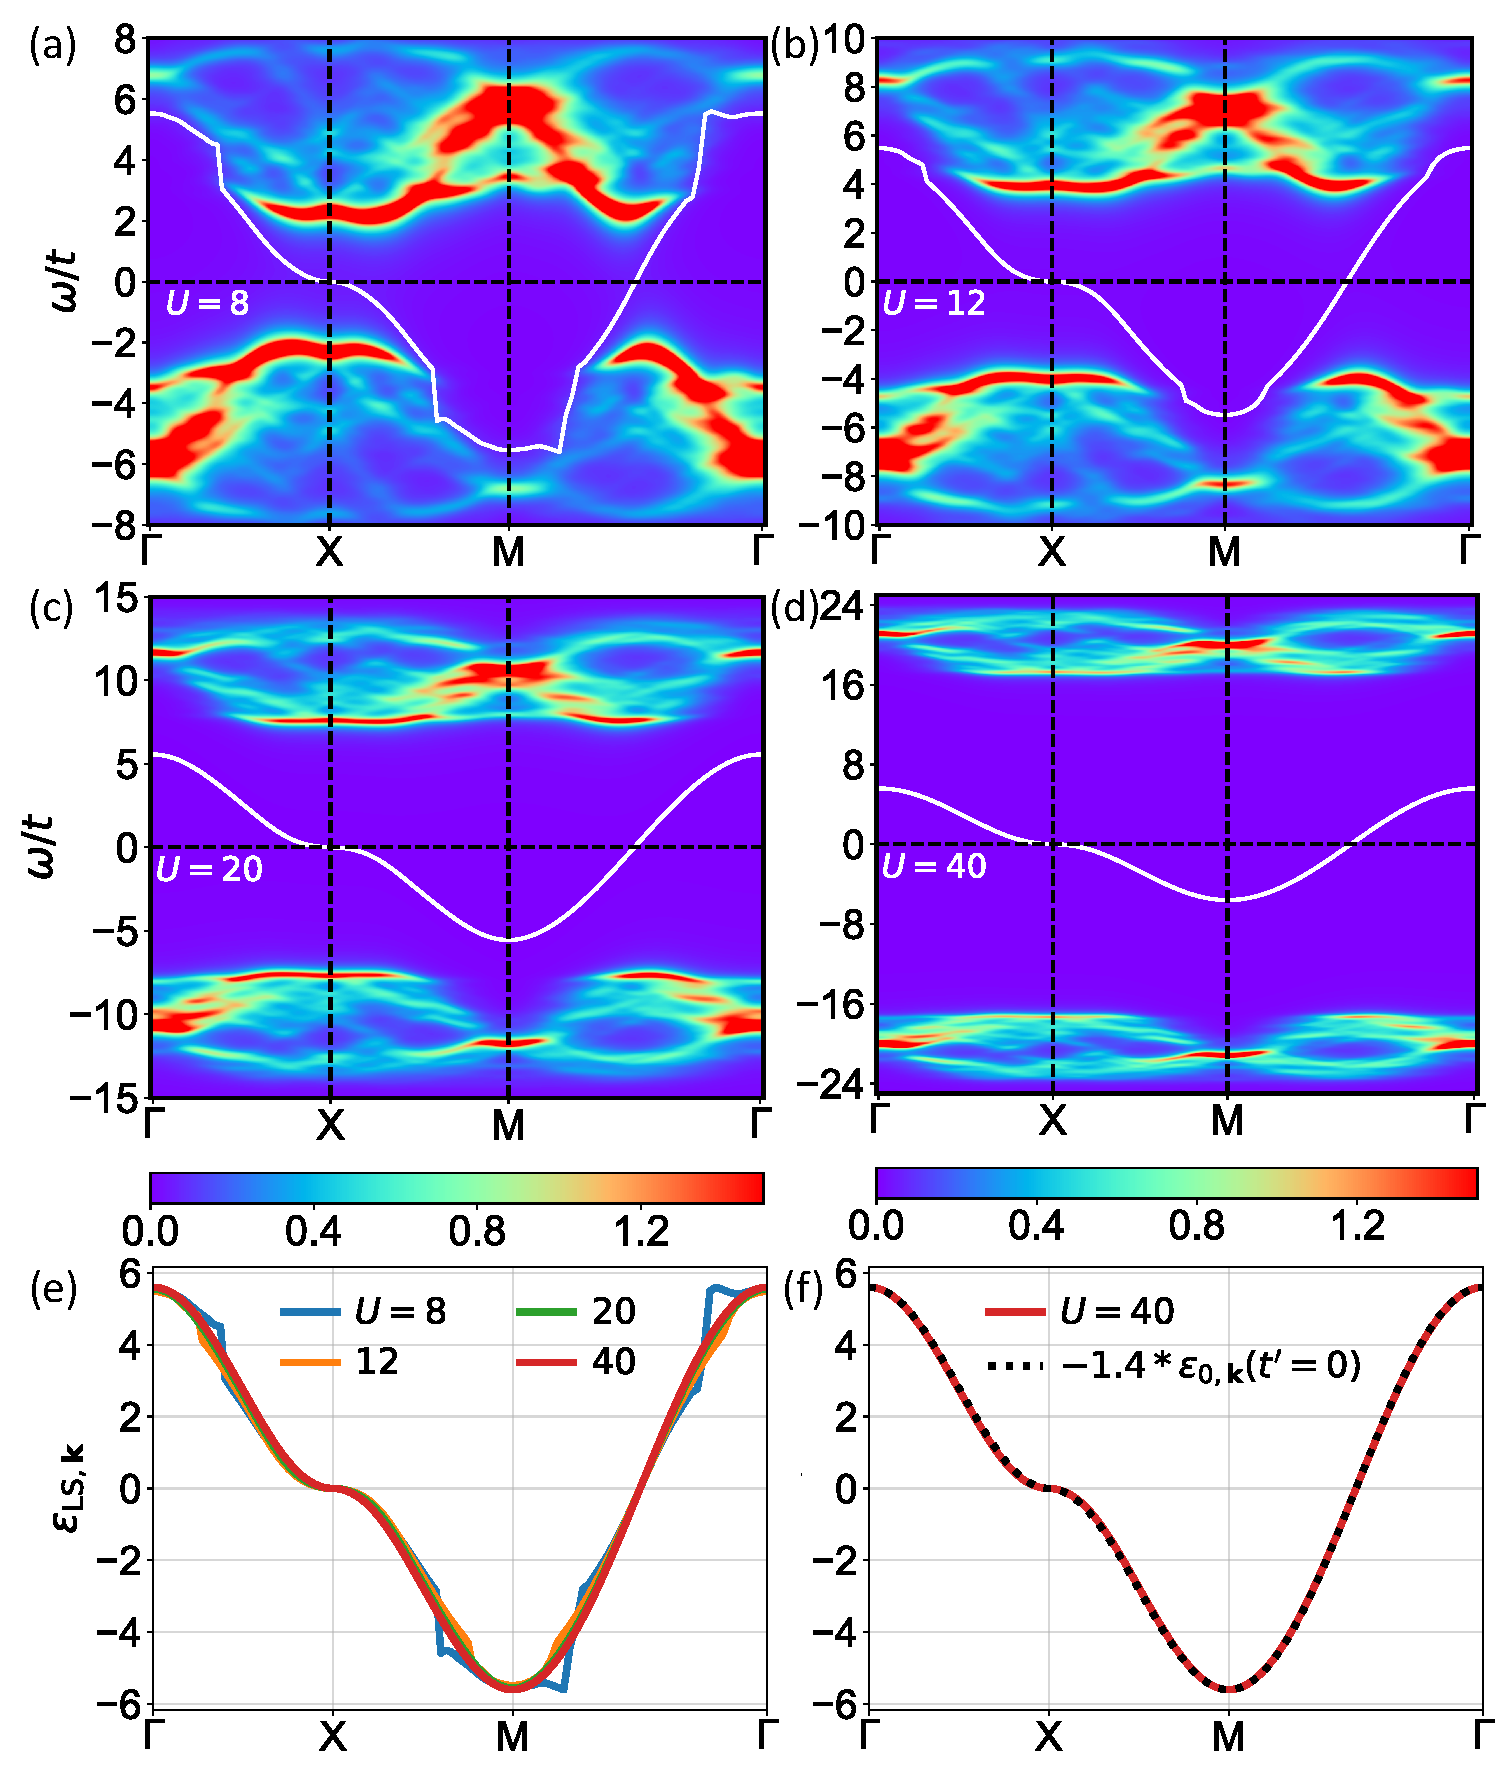
\includegraphics[width=\linewidth]{./figures/hftp0.pdf}
    \caption{Spectral function and the corresponding Luttinger surface for (a) $U/t=8$, (b) $U/t=12$, (c) $U/t=20$, and (d) $U/t=40$ from $4\times4$-OHK model with $t'=0$. Panel (e) includes the Luttinger surfaces for all values of $U$. Panel (f) shows the best fit using the non-interacting dispersion $\varepsilon_{0,k}$ for $\varepsilon_{\text{LS},k}$ at $U=40$.}
    \label{fig:hftp0}
\end{figure}

 \begin{figure}[t]
    \centering
    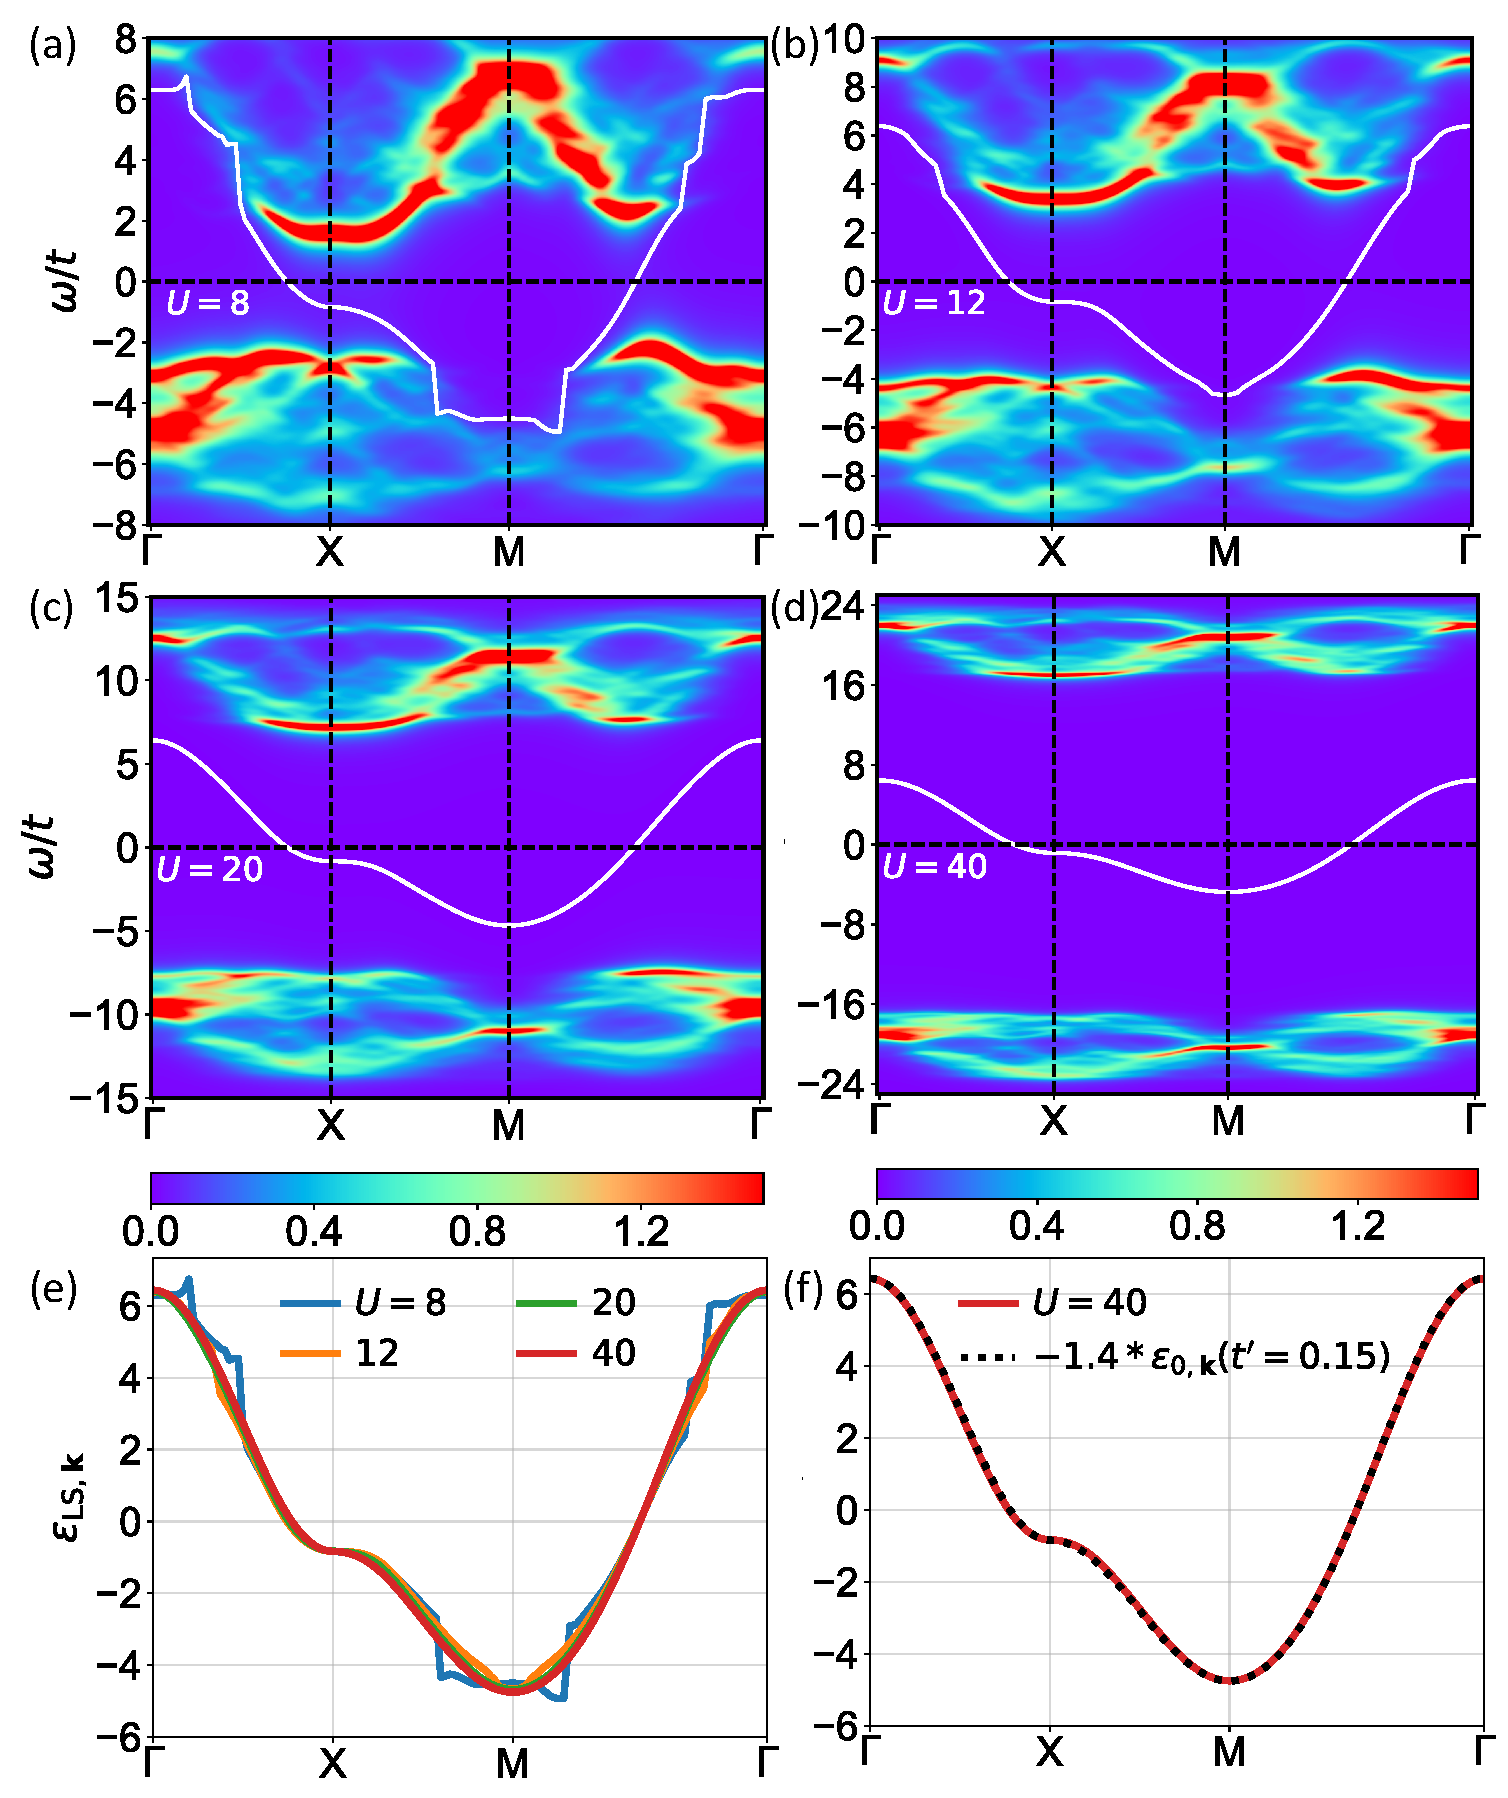
\includegraphics[width=\linewidth]{./figures/hftpn25.pdf}
    \caption{Spectral function and the corresponding Luttinger surface for (a) $U/t=8$, (b) $U/t=12$, (c) $U/t=20$, and (d) $U/t=40$ from $4\times4$-OHK model with $t'/t=-0.25$. Panel (e) includes the Luttinger surfaces for all values of $U$. Panel (f) shows the best fit using the non-interacting dispersion $\varepsilon_{0,k}$ for $\varepsilon_{\text{LS},k}$ at $U=40$.}    
    \label{fig:hftpn25}
\end{figure}

 
\bibliography{expl}
\end{document}
